\chapter{Common core}
    
\begin{itemize}
  \item In~\cite{MaslovSDM2016} we introduced Pccf and investigated its statistical properties.We introduced Pccf and applied it with the naive threshold based detector.
  \item In~\cite{MaslovIJCNN2017} We introduced uncertainty factor and applied Pccf with Bayesian detector.
  \item In~\cite{Maslov2021}We added detection delay as performance metric, improved Pccf, and applied it with CUSUM detector and investigated CUSUM specific properties.
\end{itemize}

% Three section to be joined
\section{PCCF for any distribution}

Here we introduce periodic and recurrent changes and define binary performance metrics when applied for change detection problem.

In this study we analyze how and under which conditions the performance of online change detectors can be improved for detecting recurrent changes:
\begin{itemize}	\setlength\itemsep{0pt}
    \item We define a predictive change confidence function (PCCF) for modelling recurrent changes and predicting times of changes in the future. We derive the exact analytical expression for PCCF under Gaussian data distribution.
    \item We demonstrate under which conditions taking into account recurrence information improves detection accuracy by analytically relating PCCF and time passed from the most recent confirmed change.

    \item We demonstrate how to improve the accuracy of an online change detector of user's choice by utilizing recurrence information with two simple yet generic approaches: (1)~a post-filtering of change detection output can substantially reduce the number of false alarms while preserving the same detection rate; (2)~an adaptation mechanism can be used to adjust the sensitivity of the detector online based on the change recurrence expectations.

    \item Our experimental study provides evidence that it is indeed feasible to improve performance of online change detection by utilizing recurrence information even with such simple approaches.
\end{itemize}

In subsection~\ref{subsec:chpprocess} we describe an individual change detection procedure and give definitions for recurrent and periodic changes.
In subsection~\ref{subsec:predictionprocess} we describe our approach for computing PCCF.
In subection~\ref{subsec:pccf_integration} we describe integration of PCCF with a base-level change detector.
In subsection~\ref{sec:experiments} we summarize the results of our experimental study.
Section~\ref{subsec:conclusions} concludes the paper with the summary of the contributions and future work.

\subsection{Recurrent and periodic changes}
\label{subsec:chpprocess}

The purpose of the change detection process is to detect changes in the input data stream of observations $x_t, t \in \T$ to be obtained sequentially at time moments $\T=\Collect{t_1,t_2,\dots,t_T} \equiv \Collect{t_q}_{q=1}^T$ with a constant sampling rate.
Change is identified by the moment of time when it happened.
Let us denote the sequence of changes to be detected as $\Collect{c_i }_{i=1}^k \in \T$ and an individual change from this sequence as $c_i$.
After a change occurs, we need to collect a new portion of observations during the time $\delta$ to detect the change and to assess a new probability distribution of the data.

Change detector can be considered as a binary classifier whose output for each $x_t$ is the label $\lbl{+}$ if change is alarmed, which we call a change detection event (CDE) and denote it $\Event{t}{+}$, and label $\lbl{-}$ otherwise, which we denote as  $\Event{t}{-}$.

To assess detectors' performance we define True Positive (TP), False Positives (FP), True Negatives (TN) and False Negatives (FN) as follows:
\begin{itemize}[leftmargin=*]\setlength\itemsep{0em}
    \item $\Event{t}{+}$ is TP if $\exists c_i:t-c_i<\delta$, and FP if $\nexists c_i:t-c_i<\delta$
    \item $\Event{t}{-}$ is FN if $\exists c_i:t-c_i <\delta$, and TN if $\nexists c_i:t-c_i<\delta$
\end{itemize}

Recall the real world example of a power production plant, where the task is to detect changes in the fuel mass flow signal generated by monitoring sensors.
One subtask is to detect online changes in the signal that correspond to the refueling process~\cite{PechenizkiySIGKDDExpl09}.
Consider two scenarios.
Scenario \textbf{A}: historical data indicates that refueling typically happens every day in between 7pm and 10pm (90\% of all the observed cases).
Hence, if a detector alarms a change at 11am we may conclude that most likely it is an outlier and take actions to prevent FP.
Scenario \textbf{B}: we have information that refueling is performed only when the fuel is about to run out, but we have no information that % refueling
it is performed on a daily basis.
We can observe from historical data that the average time between refueling  events is between 32 and 36 hours (90\% of all observed cases).

The two scenarios differ in possibilities to anticipate the next change point.
In scenario \textbf{A} we assume that changes are associated with time moments, which can be learned and thus known in advance (e.g.\ end of the day), while in scenario \textbf{B} we can relate future changes to the recently detected event(s).
Nevertheless, in both cases our intuition is to estimate the average time between changes from historical data, and use this information for determining the time periods where changes are more likely to happen in the future.

Let us denote by $p(c|\theta)$ a probability mass function (Pmf) defined on a discrete set of time moments $\T$ parameterized by vector $\theta$ holding information about expected distance between consecutive changes (e.g.\ the average and standard deviation).
By $p(c_i=t|\theta)$ we denote Pmf for a change $c_i$ to happen at time $t$. Recurrent and periodic changes are defined as follows.
\begin{definition}
\label{def:periodicdefinition}
Changes $\Collect{c_i}_{i=1}^k$ are periodic if
\begin{equation}
p(c_{i+1} = t|\theta) = p(c_1 = t - i w \: | \: \theta), i \in \mathbb{Z},
\label{eq:procwithrefs}
\end{equation}
where $c_1$ is the time of the first change and $w$ is a time range within which we expect the next change.
\end{definition}
Definition~\ref{def:periodicdefinition} corresponds to the case \textbf{A} and states that Pmf of a periodic change $c_{i+1}$ is a Pmf of the change $c_1$ shifted along the time axis by  $i w$.
In the power plant example, refueling happens every day in the evening, i.e.\ $i w$ is the beginning of the $i^{th}$ day and $w = 24$ hours.
\begin{definition}
\label{def:recurrentdefinition}
Changes $\Collect{ c_i }_{i=1}^k$ are recurrent if
\begin{equation}
p(c_{i+1} = t \: | \: \theta) = p(c_1 = t - c_{i} \: | \: \theta),
\label{eq:procnorefs}
\end{equation}
where
$c_1$ is the time of the $1^{st}$ change and
$c_i$ is the time of the $i^{th}$ change.
\end{definition}
Definition~\ref{def:recurrentdefinition} corresponds to the case \textbf{B} and states that Pmf of the change $c_{i+1}$ is a Pmf of the change $c_1$ shifted along the time axis by time of the $i^{th}$ change $c_i$.

\subsection{Online detection of recurrent changes}
\label{subsec:predictionprocess}

\begin{definition}
\label{def:confidencefunc}
PCCF is the probability to observe \textit{any} a recurrent change out of sequence of all possible changes $c \in \Collect{ c_i }_{i=1}^k$ at any given time moment $t$:
\begin{equation}
\mathcal{P}(t \: | \: \theta) = \sum_{i=1}^{k} p(c_i = t \: | \: \theta).
\end{equation}
\end{definition}
Next we demonstrate how to compute PCCF for recurrent (Scenario \textbf{B}) and periodic (Scenario \textbf{A}) changes, and update it using time stamps of changes $t_s$ confirmed by an online confirmation mechanism.
We show under which conditions recurrence information in a form of the average time between changes and its standard deviation $\theta = (\mu, \sigma)$ is beneficial for improving the detection accuracy.

\subsection{PCCF for periodic changes.}
The number of periodic changes $k$, which have happened until now (time $t$), can be calculated using the integer division operation:
\begin{equation}
k = \mathbf{ div }(t,w).
\end{equation}
Using Definition~\ref{def:periodicdefinition}~and~\ref{def:confidencefunc} and omitting $\theta$ we can write
\begin{equation}
\mathcal{P}(t) = \sum_{j=1}^{k = \mathbf{div}(t,w)} p(c_1 = t - (j-1) w).
\label{eq:pccf_periodic}
\end{equation}
If each $p(c_j)$ is defined only within the time interval $(jw-w, j w]$
(e.g.\ $w$ stands for the duration of the day, and we expect every change in a sequence to happen only within the next day) then PCCF will be given only by the last member of the sum in~\Eq{eq:pccf_periodic}.
An example of such PCCF is illustrated in Figure~\ref{fig:periodicexample}.
\begin{figure}[htb!]
\centering
\includestandalone[width=0.40\textwidth]{articles/pics/sdm_paper/PeriodicalEvents}
\caption{
An example of PCCF function for periodic events with $w=24$h, $i w = (24, 48, 72, \dots)$.}
\label{fig:periodicexample}
\end{figure}

\subsection{PCCF for recurrent changes.}
According to Definition~\ref{def:recurrentdefinition} Pmf of the change $c_{i+1}$ is conditioned on the time of the $i^{th}$ change $c_i$.
Following the sum rule for probability\footnote{$P(x) = \sum_{y} P(x|y) p(y)$} in order to compute Pmf of $c_{i+1}$ we need to consider all possible time locations of $c_i$.
\begin{equation}
p(c_{i+1} = t) = \sum_{\tau = i}^{t-1} p(c_{i+1}=t \: | \: c_i = \tau) p(c_i = \tau).
\label{eq:sum_rule_recurrent}
\end{equation}
PCCF is a sum over the total number of possible changes by the time moment $t$:
\begin{eqnarray}
\notag
\mathcal{P}(t) & = &  \sum_{i=1}^{t} \sum_{\tau = i}^{t-1} p(c_{i+1} = t | c_{i} = \tau)  p(c_{i} = \tau) \\
& = & \sum_{i=1}^{t} \sum_{\tau = i}^{t-1}
p(c_{1} = t - c_{i})  p(c_{i} = \tau).
\label{eq:pccf_recurren_1}
\end{eqnarray}

\subsection{Numerical PCCF computation procedure.}
Figure~\ref{fig:cascades} shows a toy example of PCCF calculation for every moment of the recurrent change detection process of time length $T=5$, i.e. $\T=\Collect{1,2,3,4,5}$.
\begin{figure}[htb!]
\centering
\includestandalone[width=0.40\textwidth]{articles/pics/sdm_paper/Cascades}
\caption{
%Trellis structure~\cite{mackay2007}
Possible times of recurrent changes.
Black dots indicate the times at which the $i^{th}$ change may have appeared with non-zero probability.
}
\label{fig:cascades}
\end{figure}
Pmf for the first change $p(c_1) = [p_1, p_2, p_3, p_4, p_5]$ is depicted by the first column of the nodes which are all black since the first change can occur at any moment $t \in [1,5]$.
According to \Eq{eq:sum_rule_recurrent} Pmf for the second change is
%%Equation~\ref{eq:sum_rule_recurrent}
\begin{eqnarray}
\notag
p(c_2) &  =  &\sum_{\tau = 1}^{4} p(c_2 = t | c_1 = \tau) p(c_1 = \tau)\\
& = & \sum_{\tau = 1}^{4} p(c_1 = t - \tau) p(c_1 = \tau).
\end{eqnarray}
This sum can be equivalently written in a matrix form
\begin{equation}
p(c_2) =
\begin{bmatrix}
 p_1 & 0   &  0   & 0   \\
 p_2 & p_1 &  0   & 0   \\
 p_3 & p_2 &  p_1 & 0   \\
 p_4 & p_3 &  p_2 & p_1
\end{bmatrix}
\begin{bmatrix}
p_1\\
p_2\\
p_3\\
p_4
\end{bmatrix}.
\label{eq:second_pccf_matrix}
\end{equation}
Thus, \Eq{eq:second_pccf_matrix} gives Pmf for $c_2$ (second column in Figure~\ref{fig:cascades}).
Pmf for $c_3,c_4,c_5$ is calculated using the same procedure.
Finally $\mathcal{P}=p(c_1)+p(c_2)+p(c_3)+p(c_4)+p(c_5)$.
The online computation procedure for an arbitrary initial Pmf $p(c_1)$
is described in Algorithm~1. %~\ref{alg:pccfalg}.

\subsection{The exact PCCF for Gaussian distribution.}
Consider Gaussain distribution for the settings when  $p(x|\theta=(\mu,\sigma)) \sim 0$ for all $x \leq 0$.

\Eq{eq:sum_rule_recurrent} is a convolution of the Pmf $p(c_1)$ of the $1^{st}$ recurrent change, which is given as a boundary condition, and of the Pmf of the change $c_i$ calculated in the previous step:
\begin{eqnarray} \notag
p(c_{i+1}) & = & (p(c_1) \ast p(c_i)) [\tau] \\
& = & \sum_{\tau = 1}^{t-1} p(c_1 = t - \tau) p(c_i = \tau).
\label{eq:sum_rule_convolution}
\end{eqnarray}
The convolution of two Gaussian distributions (please see the proof in~\cite{bromiley2003products}) is
\begin{equation}
(p(x|\mu_1, \sigma_1) \ast p(x|\mu_2, \sigma_2)) = p(x| \mu_1 + \mu_2, \sqrt{\sigma_1^2 + \sigma_2^2}).
\end{equation}
PCCF for recurrent changes can be written as a t-fold convolution and computed analytically
\begin{equation}
\mathcal{P}(t) =
(
\underbrace{
p(c_1) \ast p(c_1) \ast \dots  \ast p(c_1)
}_\text{t}
)
= p(c_1)^{\ast t}.
\end{equation}
PCCF for the moment $t$ is a sum
\begin{equation}
    \mathcal{P}(t) = \sum_{l=1}^{t} \frac{1}{\sigma \sqrt{2 \pi l}} \exp \left(\frac{-(t - l \mu)^2}{2 l \sigma^2} \right)
\label{eq:gaussian_pccf}.
\end{equation}
We can calculate the limit $L$ of $\mathcal{P}(t)$ when $t \to \infty$
\begin{equation}
L = \lim_{t \to \infty} \sum_{l=1}^{\infty} \frac{1}{\sigma \sqrt{2 \pi l}} \exp\left(-\frac{(t- \mu l)^2}{2 l \sigma^2} \right).
\label{eq:gaussian_pccf_limit}
\end{equation}
We can replace $l$ by $t/\mu$ in the denominators since we are interested in the terms for which $l \sim t / \mu$ and when $t \to \infty$, $\lim_{t \to \infty}\left( \frac{1}{t} - \frac{1}{t/\mu} \right)=0$, we are making approximation error of order $(1 + o(1))$,
\begin{equation}
L = \lim_{t\to\infty} \sum_{l=1}^{\infty} \frac{\sqrt{\mu}}{\sigma\sqrt{2\pi t}} \exp\left(-\frac{\mu^3 (t/\mu- l)^2}{2t\sigma^2}\right).
\label{eq:pccf_sum_decomposed}
\end{equation}
Exponential terms corresponding to $l$, for which $|t/\mu - l| \gg \sqrt{t}$, will have small values which we can ignored.
Therefore, we need to estimate the sum consisting of the terms for $l \in [t/\mu \pm \sqrt{t}]$.
It is convenient to consider a wider interval of width $t^{3/5} > \sqrt{t}$.
Let us consider three intervals for $l$
(1) $[0, t/ \mu - t^{3/5})$,
(2) $[t/ \mu - t^{3/5}, t/ \mu + t^{3/5}]$,
(3) $(t/ \mu + t^{3/5}, \infty)$.
The components in the sum in Eq.~\ref{eq:pccf_sum_decomposed} are very small within the intervals (1) and (3) since both are bounded by $\exp(-\frac{\mu^2}{2 \sigma^2} N^{1/5})$.
Therefore, we can find the limit by estimating the sum only within the interval (2):
\begin{equation}
L = \lim_{t\to\infty} \frac{\sqrt{\mu}}{\sigma \sqrt{2\pi t}} \sum_{l=-t^{3/5}}^{t^{3/5}} \exp\left(-\frac{\mu^3 (t/\mu - l)^2}{2t\sigma^2}\right).
\label{eq:sum_before_integral}
\end{equation}
\Eq{eq:sum_before_integral} is the Riemann sum for the Gaussian integral $\int_{-\infty}^{\infty} e^{-a x^2} dx = \sqrt{\frac{\pi}{a}} $, thus
\begin{equation}
L = \frac{\sqrt{\mu}}{\sigma \sqrt{2\pi}} \int_{-\infty}^{\infty} e^{-\frac{\mu^3 x^2}{2\sigma^2}} dx = \frac{1}{\mu}.
\label{eq:pccf_limit_proof}
\end{equation}
Figure~\ref{fig:pccf_example} illustrates two Gaussian PCCF functions (Eq.~\ref{eq:gaussian_pccf}) for two cases $(\mu=10, \sigma=2)$ and $(\mu=15, \sigma=3)$.
\begin{figure}[htb!]
\centering
\includegraphics[width=0.40\textwidth]{articles/pics/sdm_paper/pccfExamples.pdf}
\caption{An example of two Gaussian PCCF functions.
}
\label{fig:pccf_example}
\end{figure}
Local extrema of the PCCF function correspond to the time moments $l \mu, l \in \mathbb{Z}$. % where $l$ is a set of positive integers.
PCCF values converge to limits as defined in \Eq{eq:pccf_limit_proof} $L=1/10$ and $L=1/15$.

\subsection{PCCF update after a confirmed change.}
Typically, a detector would have no internal means to know for sure whether $\Event{t}{+}$ is TP or FP.
If we have a feedback mechanism indicating with some time delay $D$ when a change $c_i$ did happen,
we can update PCCF to make our detector more confident about the future change points.
Given a known $c_i$, we recompute PCCF starting from that point.
An updated PCCF is depicted by the dotted line in Figure~\ref{fig:conffunction}.
In Figure~\ref{fig:conffunction} we can see an example of how PCCF oscillates having local maximums at moments $t = k \mu$ until converging to the limit $L=0.1$.
An event at the moment $t=200$ was confirmed as a change and new PCCF is calculated (dashed line).

If we do not reestimate $\theta$ then update procedure is very fast as we simply shift already computed PCCF along the time axis.
\begin{figure}[htb!]
\centering
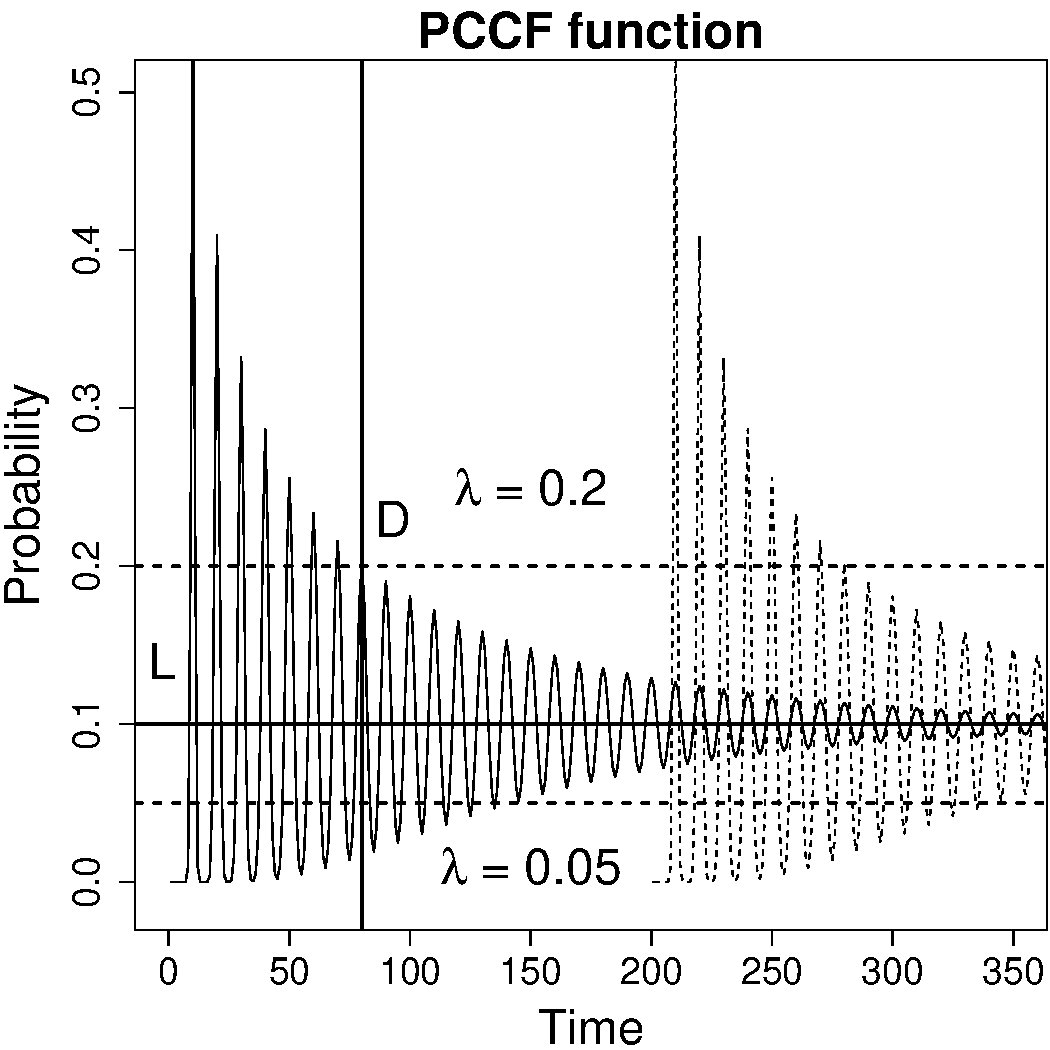
\includegraphics[width=0.35\textwidth]{articles/pics/sdm_paper/PCCF.pdf}
\caption{PCCF converges to the limit $L = 0.1$ depicted by the horizontal bold line.
Two horizontal lines $\lambda$ illustrate possible thresholds above and below the limit.
Vertical line $D$ depicts delay of change confirmation.
}
\label{fig:conffunction}
\end{figure}


\subsection{PCCF pseudo-code}
\label{subsec:pccf_pseudo_code}
In Algorithm~1, in line 11,  a zero-matrix of size $T$ is initialized with the first column filled by initial Pmf values $p(c_1)$.
In line 12 a square lower triangular matrix (Eq.~\ref{eq:second_pccf_matrix}) is generated using the function {\tt WeightsMatrix()}.
Next the probabilities for individual changes in a sequence
$\Collect{ c_i }_{i=1}^k$
are updated within the loop (line 14).
PCCF is calculated in line 15 by summing up probabilities in the columns of matrix $P$.
\begin{algorithm}
    \label{alg:pccfalg}
\begin{algorithmic}[1]
\Function{WeightsMatrix}{T,$\theta$}
    \State M = zeros(T, T);  M[1, :] = 1:T
	\For{i = 2:T}
		\For{j = i:T}
			\State M[i,j] = M[i-1, j-1]
		\EndFor
	\EndFor
	\State \textbf{return} Pmf($M^T$ $| \theta$)
\EndFunction
\\
\Function{PCCF}{$T, \theta=(\mu,\sigma)$}
\State P = zeros(T,T)
\State P[:,1] = Pmf(1:T $| \theta$) \Comment{Pmf fo the first change}
\State W = WeightsMatrix(T,$\theta$)
\For{i = 1:T-1}
	\State P[i+1:T,i+1]=W[1:T-i,1:T-i] * P[i:end-1, i]
\EndFor
\State \textbf{return} sum(P,2) \Comment{Sum of columns}
\EndFunction
\end{algorithmic}
\caption{PCCF function pseudo-code}
\end{algorithm}


\section{Pccf in Bayesian settings}
% From BLPA
Here we consider uncertainty factors.
Not too much to add. 
Mostly integration.
Pccf related section (to be merged): 

\subsection{PCCF function}
\label{subsec:pccf}
In this section we show how to compute PCCF function used to predict time locations of the recurrent changes in the future.
We consider a discrete case when observations are obtained at the discrete time moments $\langle t \rangle_{t=1}^T$ with a constant sampling rate.
Probability distribution for the discrete sets is defined using Probability mass function (\textbf{Pmf}).
As mentioned earlier we assume that changes \textit{re-}occur after `approximately' equal time intervals.
To model time intervals between consecutive changes $\langle c_i - c_{i-1} \rangle$ we use the Gaussian distribution assuming that standard deviation is small enough so that probability to observe the change $c_i$ before $c_{i-1}$ is extremely small.
\begin{definition}
    \label{def:recurrentdefinition}
    \textit{
        Changes $\Collect{c_i}_{i=1}^k$ are recurrent if
    }
    \begin{equation}
        p(c_{i+1} = t \: | \: \theta^C) = p(c_1 = t - c_{i} \: | \: \theta^C),
        \label{eq:procnorefs}
    \end{equation}
    \textit{
        where
        $\theta^C=(\mu^C,\sigma^C)$,
        $c_1$ is the time of the $1^{st}$ change,
        $c_i$ is the time of the $i^{th}$ change.
    }
\end{definition}
%
This definition corresponds to the generative model defined by
Equation~\ref{eq:recurrent_generative_model} in which every next
change $c_{i+1}$ happens after time intervals $\Delta$ which are
samples from the Gaussain distribution $N(\mu^C, \sigma^C)$.
\begin{equation}
    c_{i+1} = c_i + \Delta,~~\text{where } \Delta \sim N(\mu^c, \sigma^c)
    \label{eq:recurrent_generative_model}
\end{equation}
%
To predict future changes we introduce the notion of the
Predictive Change Confidence Function (\PCCF)~\cite{MaslovSDM2016}.
\begin{definition}
    \label{def:pccf_definition}
    \textit{
        \PCCF is a \textbf{Pmf} defined on a discrete set of time moments
        $\langle t \rangle_{t=1}^T$ giving a probability
        to observe recurrent change $\forall c \in \Collect{ c_i }_{i=1}^k$
        at the time moment $t$
    }
    \begin{equation}
        \mathcal{P}(c=t|\mu^c,\sigma^c)=\sum_{i=1}^{k} p(c_i=t|\mu^c,\sigma^c)
    \end{equation}
    \textit{
        where $p(c_i=t|\mu^c,\sigma^c)$ is a \textbf{Pmf} for an
        individual change $c_i$.
    }
\end{definition}
It is important to note that \textit{change-}events $\langle c_i \rangle$ are
independent.
Every $c_i$ can happen at any moment of time according to its
individual \textbf{Pmf} $p(c_i=t|\mu^c,\sigma^c)$.
Following the sum rule for total probability\footnote{$P(x) = \sum_{y} P(x|y) p(y)$} in order to compute Pmf of $c_{i+1}$ we need to consider all
possible time locations of $c_i$.
\begin{equation}
    p(c_{i+1} = t) = \sum_{\tau = i}^{t-1} p(c_{i+1}=t \: | \: c_i = \tau) p(c_i = \tau).
    \label{eq:sum_rule_recurrent}
\end{equation}
According to the definition~\ref{def:pccf_definition} PCCF is a sum of individual \textbf{Pmf}'s of the changes which might happen till current moment of time
\begin{eqnarray}
    \notag
    \mathcal{P}(t) & = &  \sum_{i=1}^{t} \sum_{\tau = i}^{t-1} p(c_{i+1} = t | c_{i} = \tau)  p(c_{i} = \tau) \\
    & = & \sum_{i=1}^{t} \sum_{\tau = i}^{t-1}
    p(c_{1} = t - c_{i})  p(c_{i} = \tau).
    \label{eq:pccf}
\end{eqnarray}
Right side of the Equation~\ref{eq:sum_rule_recurrent} is a convolution for the Pmf $p(c_1)$ of the $1^{st}$ recurrent change and of the Pmf of the change $c_i$ computed in the previous step
\begin{eqnarray} \notag
    p(c_{i+1}) & = & (p(c_1) \ast p(c_i)) [\tau] \\
    & = & \sum_{\tau = 1}^{t-1} p(c_1 = t - \tau) p(c_i = \tau).
    \label{eq:sum_rule_convolution}
\end{eqnarray}
The convolution of two Gaussian distributions is also Gaussian distribution
\begin{equation}
    (p(x|\mu_1, \sigma_1) \ast p(x|\mu_2, \sigma_2)) = p(x| \mu_1 + \mu_2, \sqrt{\sigma_1^2 + \sigma_2^2}).
\end{equation}
PCCF (Eq.~\ref{eq:pccf})
can be written as a t-fold convolution
\begin{equation}
\mathcal{P}(t) =
(
\underbrace{
    p(c_1) \ast p(c_1) \ast \dots  \ast p(c_1)
}_\text{t}
)
\end{equation}
% https://en.wikipedia.org/wiki/Renewal_theory !!!
% http://mathworld.wolfram.com/NormalSumDistribution.html
% Charles M. Grinstead "Introduction of probability"
% http://www.dartmouth.edu/~chance/teaching_aids/books_articles/probability_book/book.html
% https://www.dartmouth.edu/~chance/teaching_aids/books_articles/probability_book/Chapter7.pdf
%??Uncomment? = p(c_1)^{\ast t}.
%
%
%Therefore PCCF for the moment $t$ is a sum
which is equivalent to the sum
\begin{equation}
    \mathcal{P}(t) = \sum_{l=1}^{t} \frac{1}{\sigma \sqrt{2 \pi l}} \exp \left(\frac{-(t - l \mu)^2}{2 l \sigma^2} \right)
    \label{eq:gaussian_pccf}.
\end{equation}
The sum~\ref{eq:gaussian_pccf} describes renewal-reward process~\cite{cox1962renewal},~\cite{feller1968introduction}.
Using the renewal theorem~\cite{cox1962renewal}
%(Chapter 13~\cite{feller1968introduction}
we can calculate the limit of $\mathcal{P}(t)$ when $t \to \infty$
%given by expression~\ref{eq:gaussian_pccf_limit}
\begin{equation}
L = \lim_{t \to \infty} \sum_{l=1}^{\infty} \frac{1}{\sigma \sqrt{2 \pi l}} \exp\left(-\frac{(t- \mu l)^2}{2 l \sigma^2} \right) = \frac{1}{\mu}.
\label{eq:gaussian_pccf_limit}
\end{equation}
From Equation~\ref{eq:gaussian_pccf_limit} follows that PCCF converges to the constant value uniform distribution for large $t$ values.
Fig.~\ref{fig:pccf_example} illustrates two PCCF
functions (Equation~\ref{eq:gaussian_pccf}) with parameters $(\mu=10, \sigma=2)$ and $(\mu=15, \sigma=3)$.
\begin{figure}[htb!]
    \centering
    \includegraphics[width=0.40\textwidth]{images/blpa_article/pccfExamples.pdf}
    \caption{
        An example of two Gaussian PCCF functions.
        The limits are $\frac{1}{\mu^C}.$
    }
    \label{fig:pccf_example}
\end{figure}
Prior and posteriors for the PCCF's parameters are estimated and updated using the procedure described in Section~\ref{sec:data_model} describing data model.

\subsection{Uncertainty model (Data model)}
In this section we describe the data model which we use in BLPA.
There are two streams of data to be analysed.
The stream of input observations $\langle x_t \rangle$ and the stream of time intervals between changepoints  $\langle c_i - c_{i-1} \rangle$.
The first stream is used to detect changes and therefore to produce the second stream.
The stream of changes maybe updated by the outer sources providing additional information about time location of the changes.
E.g. there is a process running in parallel with the main detector which can run additional change-detection processes over collected data to identify locations of the changes in the past more precisely.
The stream of changepoints is used to predict future changepoints in order to adjust detector's settings to achieve a better performance.
Further, data $D$ is either input data stream of observations $\langle x_t \rangle$ or data stream of time intervals between consecutive changepoints $\langle c_i - c_{i-1} \rangle$.
In this section we describe a data model for $D$ common both for input signal and sequence of time intervals between changepoints.

Data $D$ is assumed to be generated by a Gaussian distribution with an unknown mean and variance.
We denote elements of $D$ by $\xcommon \in D$ with mean and variance $(\mucommon, \sigmacommon)$.

\subsection{Prior distributions.}
Following the notations in~\cite{JordanChapter9}, we use a \emph{normal-gamma} prior for $\mucommon$ and $\sigmacommon$:
%
\begin{align}
    \xcommon &\sim N(\mucommon,\taucommon),~~\taucommon=(1/\sigmacommon)^2\\
    \mucommon &\sim N(\muzerocommon,\kappazerocommon \taucommon)\\
    \taucommon &\sim Gamma(\alphazerocommon,\betazerocommon)
    \label{eq:theta_normal_gamma}
\end{align}
%
where $(\alphazerocommon, \betazerocommon, \muzerocommon,
\kappazerocommon)$ are hyperparameters.
%
The value $\taucommon$ is also named
\emph{precision}~\footnote{Further we use $\sigma$ and $\tau$
    parameters interchangeably.}.
%
The likelihood of data $D=\langle \xcommon \rangle$ is
%
\begin{equation}
P(D|\mucommon, \taucommon) = \Big(\frac{\taucommon}{2\pi} \Big)^{n/2}  \exp \Big (-\frac{\taucommon}{2}\sum_{i=1}^{n}(\xcommon-\mu)^2 \Big)
\end{equation}
%
The joint conjugate prior for parameters $(\mucommon,\taucommon
)$ is the defined \emph{normal-gamma} (\textit{NG}) distribution:
%
\begin{align}
    &P(\mucommon,\taucommon | \muzerocommon,\kappazerocommon,\alphazerocommon,\betazerocommon) =  N(\muzerocommon,\kappazerocommon \taucommon) Gamma(\alphazerocommon,\betazerocommon)\\
    &=\frac{1}{Z}\taucommon^{1/2}\exp\Big(-\frac{\kappazerocommon \taucommon}{2}(\mucommon-\muzerocommon)^2\Big)\taucommon^{\alphazerocommon-1}e^{-\taucommon \betazerocommon}\\
    &=\frac{1}{Z}\taucommon^{\alphazerocommon-1/2}\exp\Big(-\frac{\taucommon}{2}[\kappazerocommon(\mucommon-\muzerocommon)^2+2\betazerocommon]\Big)
\end{align}
%
where $Z=\frac{\Gamma(\alphazerocommon)}{\betazerocommon^{\alphazerocommon}}\Big(\frac{2\pi}{\kappazerocommon}\Big)^{1/2}$
is the normalized factor.

\subsection{Posterior distributions}
%Therefore,
The posterior can be derived as
%
\begin{align}
    P(\mucommon,\taucommon|D) &\varpropto P(\mucommon,\taucommon|\muzerocommon,\kappazerocommon,\alphazerocommon,\betazerocommon)P(D|\mucommon, \taucommon)\\
    &\propto N(\mucommon_n, \kappacommon_n \taucommon) Gamma(\alphazerocommon+n/2,\betacommon_n)
    \label{eq:mu_tau_posterior}
\end{align}
%
which is also a \emph{normal-gamma} distribution:
%
\begin{equation}
P(\mucommon,\taucommon|D)=NG(\mucommon,\taucommon|\mucommon_n,\kappacommon_n,\alphacommon_n,\betacommon_n)
\label{eq:mu_tau_prior}
\end{equation}
%
with the parameters
%
\begin{align}
    \mucommon_n&= \frac{\kappazerocommon}{\kappazerocommon + n} \muzerocommon + \frac{n}{\kappazerocommon + n} \bar x\\
    \kappacommon_n&= \kappazerocommon + n\\
    \alphacommon_n&= \alphazerocommon + n/2 \\
    \betacommon_n&= \betazerocommon+\frac{1}{2}\sum_{i=1}^{n}(\xcommon-\bar{x})^2+\frac{\kappazerocommon n(\bar{x}-\muzerocommon)^2}{2(\kappazerocommon+n)}
    \label{eq:update_rule}
\end{align}
where $\bar{x}=\frac{1}{n}\sum_{i=1}^{n}\xcommon$ is the mean of sampled data.
The posterior distribution for $\taucommon$ is obtained by
integrating Equation~\ref{eq:mu_tau_prior} over $\mu$
(See~\cite{JordanChapter9}) --
\begin{multline}
    p(\taucommon | D, \muzerocommon, \kappazerocommon, \alphacommon, \betacommon) \varpropto\\
    Gamma(\alphacommon + n/2, \betacommon + \frac{1}{2} \sum_{i=1}^n (\xcommon-\bar{x})^2 +
    \frac{\kappacommon \kappazerocommon}{2(\kappacommon + \kappazerocommon)} (\bar{x} - \muzerocommon)^2 ))
    \label{eq:kappa_posterior}
\end{multline}
Given the updated parameters
$\theta=(\alpha_0, \beta_0, \mu_0, \kappa_0)$ using the rules~\ref{eq:update_rule} ,
the predictive distribution for a new data $x_{\text{new}}$ is
\begin{multline}
    p(x_{\text{new}} | \pmb{x}, \mu, \kappa, \alpha, \beta) = \\
    \int p(x_{\text{new}} | \mu, \tau) p(\tau | \pmb{x}, \mu_0, \kappa_0, \alpha, \beta) d \tau
    \label{eq:predictive_distribution}
\end{multline}
where
\begin{equation}
p(x_{\text{new}} | \mu, \tau) = (\frac{\tau}{2 \pi})^{1/2} e^{-\frac{\tau}{2} (x-\mu)^2} d \tau
\end{equation}
and $p(\tau | \pmb{x}, \mu_0, \kappa_0, \alpha, \beta)$ is given by~\ref{eq:kappa_posterior}.
Integral~\ref{eq:predictive_distribution} is a Pearson type VII distribution (Equation~\ref{eq:predictive_distribution2}) which is
equivalent of the non-standardized Student's t-distribution.
\begin{equation}
p(x_{\text{new}})=\frac{1}{\alpha B(m - 1/2,1/2)} \Big (  1 + \Big (\frac{x_{n+1} - \lambda}{\alpha} \Big )^2 \Big )^{-m}
\label{eq:predictive_distribution2}
\end{equation}
where
\begin{align}
    m &= \alpha_0 + (n+1)/2\\
    %
    \alpha &= A \sqrt{ \sum_{i=1}^{n} x_i^2 + \kappa_0 \mu_0^2 - \frac{( \sum_{i=1}^{n} x_i + \mu_0 \kappa_0 )^2}{n + \kappa_0} + 2 \beta_0 }\\
    %
    A &= \sqrt{\frac{n+1+\kappa_0}{n+\kappa_0}}\\
    %
    \lambda &= \frac{\sum_{i=1}^n x_i + \mu_0 \kappa_0}{n + \kappa_0}
    \label{eq:posteriro_parameters}
\end{align}
Predictive distribution~\ref{eq:bd_marginal_predictive} in case
of this data model is given by Equation~\ref{eq:predictive_distribution2}.
Please see detailed calculations:

\noindent
\textbf{Marginal predictive distribution} $p(x_{n+1}|x_1,...,x_n)$ can be found as
\begin{align}
\label{eq:post1}
    &p(x_{n+1}|x_1,...,x_n)\\\nonumber
    &=\frac{ \int_{\tau\in \mathbb{R}^+} \int_{\mu\in \mathbb{R}}p(x_1,....,x_{n+1}|\mu,\tau) p(\mu,\tau)d\mu d\tau}{ \int_{\tau\in \mathbb{R}^+} \int_{\mu\in\mathbb{R}}p(x_1,....,x_{n}|\mu,\tau) p(\mu,\tau)d\mu d\tau}.
\end{align}
Assuming the Gaussian distribution 
\begin{equation}
    p(x|\mu,\tau)=\frac{\sqrt{\tau}}{\sqrt{2\pi}} e^{-\frac{\tau}2 (x-\mu)^2}
    \label{eq:gauss_appendix}
\end{equation}
the probability $p(x_1,....,x_{n}|\mu,\tau) p(\mu,\tau)$ is
\begin{align}\label{eq:prob1}
    \left(\frac{\sqrt{\tau}}{\sqrt{2\pi}}\right)^{n}\times &\exp\left(-\frac{\tau}{2}\sum_{i=1}^{n} (x_i-\mu)^2\right) \tau^{\alpha_0-1/2}\\\nonumber &\times\exp\left(-\frac{\tau}2 \left(\kappa_0(\mu-\mu_0)^2+2\beta_0\right) \right)
\end{align}
where an expression in the exponent is 
\begin{align}
    &-\frac{\tau(n+\kappa_0)}{2}\sum_{i=1}^{n} \left(\mu-\frac{\sum_{i=1}^{n} x_i+\mu_0 \kappa_0}{n+\kappa_0}\right)^2\\\nonumber &-\frac{\tau}{2} \left(\sum_{i=1}^{n} x_i^2 + \kappa_0\mu_0^2 - \frac{(\sum_{i=1}^{n}x_i +\mu_0 \kappa_0)^2}{n+\kappa_0}+2\beta_0\right),
\end{align}
Therefore %from where
\begin{align}
    &p(x_1,....,x_{n}|\mu,\tau) p(\mu,\tau)\\\nonumber
    =& \left(\frac{1}{\sqrt{2\pi}}\right)^{n-1} \frac{\Gamma(\alpha_0+n/2)}{\sqrt{n+\kappa_0}} \left(\frac{\hat{b}_n}2\right)^{-\alpha_0+n/2}\\\nonumber \times &\GammaDistr(\tau|\alpha_0+n/2,\hat{a}_n/2) \mathcal{N}(\mu|\hat{\mu}_n,\hat{\sigma}^2_n)
\end{align}
where posterior parameters estimates $\hat{a}_n, \hat{\mu}_n, \hat{\sigma}^2_n$ are
\begin{align}
    &\hat{a}_n = \left(\sum_{i=1}^{n} x_i^2 + \kappa_0\mu_0^2 - \frac{(\sum_{i=1}^{n}x_i +\mu_0 \kappa_0)^2}{n+\kappa_0}+2\beta_0\right),\\\nonumber &\hat{\mu}_n = \frac{\sum_{i=1}^{n}x_i+\mu_0 \kappa_0}{n+\kappa_0},\ \hat{\sigma}^2_n = \frac{1}{\tau(n+\kappa_0)}.
\end{align}
Therefore the integral in the numerator in Equation~\ref{eq:post1} is
\begin{align}
    &\int_{\tau\in \mathbb{R}^+} \int_{\mu\in \mathbb{R}}p(x_1,....,x_{n+1}|\mu,\tau) p(\mu,\tau)d\mu d\tau\\\nonumber
    =& \left(\frac{1}{\sqrt{2\pi}}\right)^{n-1} \frac{\Gamma(\alpha_0)}{\sqrt{n+\kappa_0}} \left(\frac{\hat{a}_n}2\right)^{-(\alpha_0+n/2)}
\end{align}
and integral~\ref{eq:post1} can be expressed as
\begin{align}
    &\frac{\sqrt{n+\kappa_0}}{\sqrt{n+1+\kappa_0}\ B(\alpha_0+n/2,1/2)} \frac{\hat{a}_n^{\alpha_0+n/2}}{\hat{a}_{n+1}^{\alpha_0+(n+1)/2}}\\\nonumber
    =&\frac{\sqrt{n+\kappa_0}}{\sqrt{n+1+\kappa_0}\ B(\alpha_0+n/2,1/2)} \left(\frac{\hat{a}_{n+1}}{\hat{a}_n}\right)^{-(\alpha_0+(n+1)/2)} \hat{a}_n^{-1/2}.
\end{align}
Noticing that
\begin{align}
    &\frac{\hat{a}_{n+1}}{\hat{a}_n} = 1+ \frac{n+\kappa_0}{\hat{a}_n(n+1+\kappa_0)}\\\nonumber \times &\left(x_{n+1}^2 - \frac{2x_{n+1}\left(\sum_{i=1}^n x_i +\mu_0 \kappa_0\right)}{n+\kappa_0}
    + \frac{\left(\sum_{i=1}^n x_i +\mu_0 \kappa_0\right)^2}{(n+\kappa_0)^2}\right)
\end{align}
\textbf{marginal predictive distribution} is 
\begin{align}
    &p(x_{n+1}|x_1,...,x_n)\\\nonumber =& \frac{1}{\hat{b}_n B(\alpha_0+n/2,1/2)} \left(
1+\frac{(x_{n+1}-\lambda)^2}{\hat{b}_n^2}\right)^{-(\alpha_0+(n+1)/2)},
\end{align}
where coefficients are
\begin{equation}
    \hat{b}_n = \frac{\sqrt{(n+1+\kappa_0)\hat{a}_n}}{\sqrt{(n+\kappa_0)}},\ \lambda = \frac{\sum_{i=1}^n x_i +\mu_0 \kappa_0}{n+\kappa_0}.
\end{equation}


\section{From Journal}
From~\cite{Maslov2021}.

Adaptive learning in concept drift.
Predictability of events in the data stream.
Sums of independent random variables.
Recurrency is a form of predictability.

If change points are expected to reoccur in the input signal, then this prior information can be used to approximate prediction time intervals, or regions of interest (ROI), where changes are most likely to appear in the future.
Once calculated, and if predictions are correct, then this information can further be used to reduce the false alarm rate of the change detection process, and potentially to reduce detection delays too.
FA rate can be decreased just by disregarding detections outside prediction intervals, and the detection delay can be decreased by increasing sensitivity of the detector within prediction intervals.
But, as mentioned, if sensitivity is increased, then probability of FA events will also increase.
Possibility of decreasing detection delays in the presence of prediction interval is a subject of Experiments section.
We describe next how to calculate prediction intervals for reoccurring change points.

To calculate ROIs for recurrent change points we use a prediction confidence change function (Pccf) proposed in our previous work~\cite{MaslovSDM2016}, where it was calculated using convolutions.
Below we calculate Pccf for several commonly used distributions of inter-arrival times values using moment generating functions, what is a more concise way than when using convolutions.
Let's start with definitions.
\begin{definition}
	Change points $t_i^{\text{c}}$ are recurrent if their inter-arrival times $t_{i}^{c} - t_{i-1}^{c}$
	are i.i.d.\ from the same probability distribution.
	E.g., $t_{i}^{c} - t_{i-1}^{c} \sim \mathbb{N}(\mu, \sigma)$ if $\sigma$ is small.
\end{definition}
Pccf function value at time moment $t_i$ is a probability estimator of recurrent change point to occur at this time moment.
Pccf can be represented as a matrix~\ref{eq:pccf_matrix} in which elements at row $k$ and column $i$ are probability estimates for change point $t_k^{\text{c}}$ to appear at time moment $t_i$.
\begin{equation}~\label{eq:pccf_matrix}
	\text{PCCF}_{k,i} \equiv P(t_{k}^{\text{c}} = t_i) % \: \forall \:  k, i \in [1,\dots,N
\end{equation}
When calculating ROIs we are interested in total probability of any changepoint occurring at every time moment within prediction horizon.
Since events $t_k^{\text{c}} = t_i$ are disjoint we need to sum up rows of the matrix $\text{PCCF}_{k,i}$
\begin{equation}~\label{eq:pccf_vector}
	\text{PCCF}_{i \in 1:N} = \sum_{k=1}^{N} P(t_k^{\text{c}} = t_i) \equiv \sum_{k=1}^{N} \text{PCCF}_{k,i}
\end{equation}
Further by Pccf we call the vector given by Equation~\ref{eq:pccf_vector}.

The sum~\ref{eq:pccf_vector} can be calculated using the notion of moment generating function (Mgf).
As an example, let's assume a Gaussian distribution for inter-arrival times, i.e. $t_{i}^{\text{c}} - t_{i-1}^{\text{c}} \sim \mathbb{N}(\mu, \sigma)$,
with $\sigma$ small enough so that every next change can not happen before the previous one.
For example, if $\mu=60$ seconds and standard deviation is $\sigma=5$ seconds then, using Chebyshev's inequality~\ref{eq:chebyshev_ineq}, probability of
$\mathbb{P}(|t_{i}^{\text{c}} - t_{i-1}^{\text{c}}| \geq 60) \leq 0.007$.
\begin{equation}\label{eq:chebyshev_ineq}
	\mathbb{P}(|X-\mu| \geq k \sigma) \leq \frac{1}{k^2} 
\end{equation}
By definition, Mgf, or Laplace transform, of random variable $X$ is~\ref{eq:mgf}
\begin{equation}\label{eq:mgf}
	M_{X}(t) = \mathbb{E}(e^{t X}), \: t \in \mathbb{R}
\end{equation}
Using the property that expected value of the product of two independent random variables is the product of their expected values $\mathbb{E}(X \dot Y)=\mathbb{E}(X)\mathbb{E}(Y)$, Mgf of the sum of independent random variables is a product of individual Mgfs (Equation~\ref{eq:mgf_of_sum}).
\begin{equation}\label{eq:mgf_of_sum}
	M_{X+Y}(t) = \mathbb{E}(e^{t (X+Y)}) = \mathbb{E}(e^{t X}) \mathbb{E} (e^{t Y}) \equiv M_{X}(t) M_{Y}(t)
\end{equation}
For the Gaussian distribution Mgf is $\exp{(\mu t + \frac{\sigma^2 t^2}{2})}$ and therefore
\begin{equation}\label{eq:mgf_gauss}
	M_{X+Y}^{\text{Gaussian}}(t)  = \exp \Big ((\mu_X + \mu_Y) t + \frac{(\sigma_X^2 + \sigma_Y^2) t^2}{2} \Big )
\end{equation}
But~\ref{eq:mgf_gauss} is Mgf of the Gaussian distribution with parameters $\mu=\mu_1+\mu_2$ and $\sigma=\sqrt{\sigma_X^2 + \sigma_Y^2})$.
Therefore if probability distribution of the first change point is $t_1^{\text{c}} \sim \mathbb{N}(\mu, \sigma)$ then $t_2^{\text{c}} \sim \mathbb{N}(2\mu, \sigma \sqrt{2})$, etc.
And Pccf is a sum~\ref{eq:pccf_gaussian}
\begin{equation}\label{eq:pccf_gaussian}
	\text{PCCF}^{\text{Gaussian}} \equiv \sum_{k=1}^N \mathbb{N}(k \mu, \sqrt{k} \sigma)
\end{equation}

Using the same logic it is straightforward to calculate Pccfs for Exponential and Gamma distributions (Table~\ref{table:pccfs}).
\begin{table}[!htb] \caption{Pdf's for distributions of inter-arrival times.}\label{table:pccfs}
	\begin{center}
		\begin{tabular}{|l|l|c|c|}
			\hline
			Distribution & Mgf & PDF of the $k$-th event & PCCF  \\[5pt]
			\hline
			Gaussian & $\exp{ (\mu t + \frac{\sigma^2 t^2}{2}) }$ & $\mathcal{N}(k \mu, \sqrt{k} \sigma)$ & $\sum_{k=1}^N \mathcal{N}(k \mu, \sqrt{k} \sigma)$ \\
			Gamma $\Gamma(\alpha, \lambda)$ & $\Big ( \frac{1}{1- \lambda t} \Big )^{\alpha}$ & $\Gamma(k \alpha, \lambda)$ & $\sum_{k=1}^N \Gamma(k \alpha, \lambda)$\\
			Exponential & $\frac{\lambda}{\lambda - t}$ & $\Gamma(k, \lambda)$ & $\sum_{k=1}^N \Gamma(k, \lambda)$\\
			\hline
		\end{tabular}
	\end{center}
\end{table}
Figure~\ref{fig:pccf_example} depicts Gaussian Pccf.
Prediction intervals (ROI) can be calculated by applying a threshold value for Pccf and then ROIs will be determined by time moments when Pccf exceeds this threshold.
In this way we would take into account uncertainty in the predictions for $k$-th change points which will increase as $\sqrt{k} \sigma$ (Equation~\ref{eq:pccf_gaussian}).
Another way is to use the property that Pccf extremums are equally spaced (Equation~\ref{eq:rois})~\cite{MaslovSDM2016} by time intervals $\mu$.
After estimating $\mu$ between changes and choosing the number of change points $k$ to predict and ROIs width prediction interval are determined by Equation~\ref{eq:rois}.
\begin{equation}\label{eq:rois}
	\text{ROI}s = (\mu \pm \text{ROI}_{\text{Width}}, 2 \mu \pm \text{ROI}_{\text{Width}}, \dots , k \mu \pm \text{ROI}_{\text{Width}}).
\end{equation}
\begin{figure}[!htb]
	\centering
	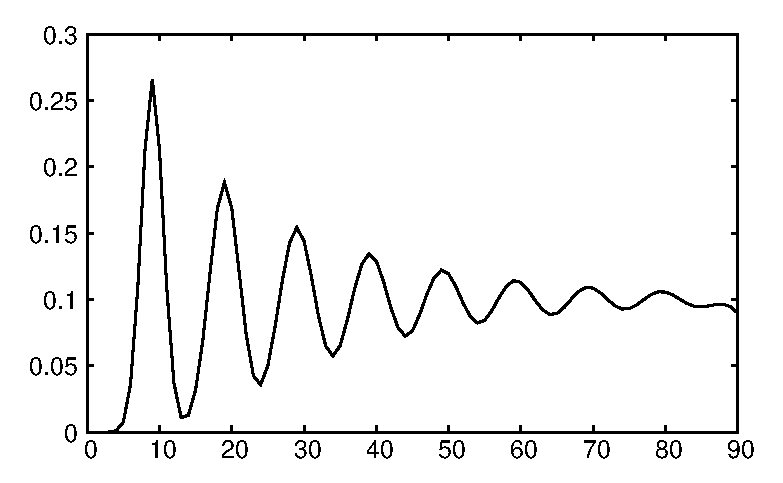
\includegraphics[width=0.7\textwidth]{images/example_pccf.eps}
	\caption{Pccf example}\label{fig:pccf_example}
\end{figure}

